\begin{figure*}[t]
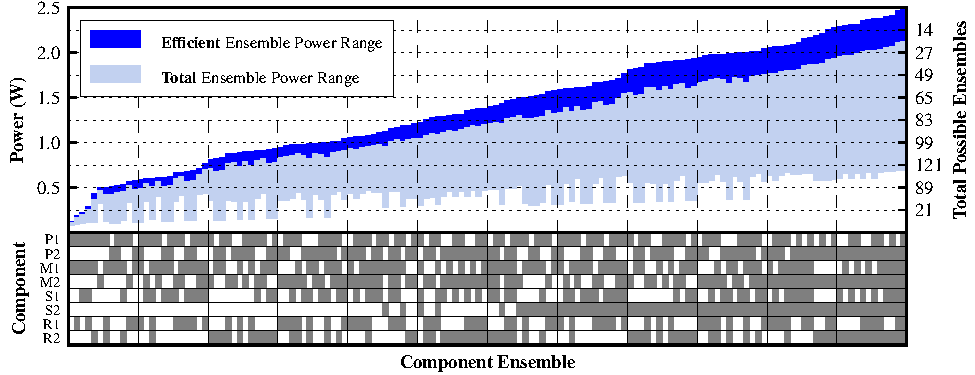
\includegraphics{./figures/componentgraph.pdf}

\caption{\small \textbf{Power envelopes of all 144 2x2x2x2 device component
ensembles.} Ensembles are sorted by increasing maximum power draw. For each
ensemble, the bottom shows which components are active and the top displays
the power envelope. The top 80\% of the envelope --- the efficient operating
range --- is drawn in dark blue. The right axis counts the total number of
ensembles that might draw that much power: e.g., there are
121 ensembles that could consume 0.75~W, depending on the workload.}
\vspace{0.10in}
\hrule
\vspace{-0.20in}
\label{figure-componentgraph}
\end{figure*}

\section{Example Architecture and Scenario}
\label{section-architectureandscenario}

We motivate the need for power-agility using an example. To begin, we
assemble a component ensemble suitable for a mobile device.
Table~\ref{table-components} summarizes properties of the parts we chose:
eight components, two processors, memory chips, storage devices, and radios.

The relationship between power and performance is complex for each component.
Processors provide a smooth performance transition over a restricted power
envelope using DVFS, but cannot scale to zero due to leakage current that
increases as a function of the number of transistors. Memory chips have a
fixed refresh cost that scales somewhat with their size and an addition
scaling component corresponding to usage. Storage devices differ based on
whether they include spinning components: those that do not (Flash-based)
scale power roughly with usage but at presently limited in their size. Today,
very high capacity drives still use spinning platters and suffer from the
high background power draw necessary to rotate them. Radios exhibit even more
interesting power-performance variation because usage depends both on
properties of the hardware and characteristics of the protocol. 802.11 radios
can enter power-saving mode (PSM) which leverages base station infrastructure
to save client power. Bluetooth has limited range but lower power consumption
balanced between both ends of the link.

Using the components we selected allows our device to operate across a wide
power range. It its lowest-power ensemble, the device has a 75~MHz CPU and
32~MB of RAM, draws as little as 82~mW\footnote{Actual power consumption
would be higher due to system buses, memory controllers, and other components
of a complete architecture.} and is roughly-equivalent to a embedded sensor
node; in its highest-power ensemble with all components powered and active
the device has multiple cores, over 1~GB of RAM, over 320~GB of storage, Wifi
and Bluetooth. Consuming almost 2.5~W, it is similar to emerging smartphones.

In total our device can activate \textit{144 possible component ensembles}.
Figure~\ref{figure-componentgraph} shows all possibilities and the power
range associated with each, and illustrates several key observations.
\textbf{First, there is wide variation in the power usage of component
ensembles even in an architecture with only two components per class.}
Incorporating more components per class would result in even more variation.
\textbf{Second, at any overall power level there are many components
ensembles that the device can use.} A diverse set of ensembles is available
at most power points: a fast processor, small memory chip, and slow disk; a
slow processor, large memory, and a fast radio; etc. Of course, not all
possible ensembles at a given power point may be possible or make sense --- a
processor of sufficient speed may be required to drive a high-bandwidth radio
--- but, given careful component choices, we think many will. It also may not
make sense to operate a component ensemble at a power level insufficiently to
allow high levels of component activity, but given the variations in load and
availability and the potential overhead of transitions between component
ensembles we believe that devices will spend some time at the low end of
ensemble power envelopes.

We illustrate how our heterogeneous device might react to fluctuating power
availability and demand by transitioning between component ensembles in
Figure~\ref{figure-transitiongraph}. Imagine a wind-powered microserver made
available to mobile devices for task processing. Walking through the
scenario:

\begin{figure*}
\noindent\begin{minipage}[t]{0.5\textwidth}
\vspace{0pt}
{\small
\begin{tabularx}{\columnwidth}{cX}

\textbf{t} &
\multicolumn{1}{c}{\textbf{Description}}
\\ \toprule 

0 & With no tasks to process, \textbf{P1} and \textbf{M1} are idle, while
\textbf{R1} operates at low duty cycle awaiting incoming tasks.
\\

1 & 
Alerted to an incoming task, the device activates \textbf{R2} to rapidly
receive task data and \textbf{S1} to store it.
\\

2 &
When processing begins, energy usage is reconfigured by activating
\textbf{P2} and disabling \textbf{R2}.
\\

3 &
Responding to a spike in availability, task processing is accelerated by
activating \textbf{M2} and mirroring to \textbf{S2}.
\\

\end{tabularx}
}
\end{minipage}
\begin{minipage}[t]{0.5\textwidth}
\vspace{0pt}
{\small
\begin{tabularx}{\columnwidth}{cX}

& \\ \toprule 

4 &
As results start being written to disk, power usage shifts within the same
component ensemble.
\\

5 & 
When availability drops to 1~W, the device stores compressed results on
\textbf{S1}.
\\

6 &
To return results, \textbf{R3} is activated and driven using \textbf{P1}.
\\

7 &
When power availability falls again, the device disables \textbf{M3} and
switches to the smaller memory chip \textbf{M1}.
\\

8 &
Processing is complete.
\\

\end{tabularx}
}
\end{minipage}
\caption{\small \textbf{Test.} Test}
\label{table-transitions}
\vspace{0.10in}
\hrule
\vspace{-0.20in}
\end{figure*}


\begin{table}[t]
\begin{threeparttable}
{\footnotesize
\begin{tabularx}{\textwidth}{clrlXr}

\multicolumn{1}{c}{\textbf{\large{Type}}} &
\multicolumn{1}{c}{\textbf{\large{Name}}} &
\multicolumn{2}{c}{\textbf{\large{Power (mW)}}} &
\multicolumn{1}{c}{\textbf{\large{Performance}}} &
\multicolumn{1}{c}{\textbf{\large{ID}}}
\\ \toprule 

\multirow{6}{*}{\vspace{-0.15in}\textbf{CPU}} &
\multirow{2}{*}{ARM Cortex-M4\tnote{11}~\cite{cortexm4-web}} &
0.9\tnote{1} & &
75 MHz, 94 MIPS\tnote{2} &
\multirow{2}{*}{\textbf{P1}}
\\

& & &
15.6 &
300 MHz, 375 MIPS
&
\\ \cmidrule(l){2-6}

& \multirow{2}{*}{ARM Cortex-R4\tnote{11}~\cite{cortexr4-web}} &
4.6\tnote{1} & &
206 MHz, 342 DMIPS\tnote{2} &
\multirow{2}{*}{\textbf{P2}}
\\

& & &
78.8 &
620 MHz, 1030 DMIPS
&
\\ \cmidrule(l){2-6}

& \multirow{2}{*}{ARM Cortex-A9~\cite{cortexa9-web}} &
23.5\tnote{1} & &
415 MHz, 1037 DMIPS\tnote{2} &
\multirow{2}{*}{\textbf{P3}}
\\

& & &
400 &
830 MHz, 2075 DMIPS
&
\\ \toprule

\multirow{8}{*}{\vspace*{-0.15in}\textbf{Memory}} &
\multirow{2}{*}{\textbf{32~MB} ISSI SDRAM~\cite{issi32MBsdram-datasheet}} &
81 & &
Refresh only &
\multirow{2}{*}{\textbf{M1}}
\\

& & &
108 &
166 MHz
&
\\ \cmidrule(l){2-6}

&
\multirow{2}{*}{\textbf{256~MB} Micron ``Slow'' DDR2} &
239\tnote{10} & &
Refresh only &
\multirow{2}{*}{\textbf{M2}}
\\

& & &
405 &
266 MHz, 478Mtps
&
\\ \cmidrule(l){2-6}

&
\multirow{2}{*}{\textbf{1~GB} Micron ``Slow'' DDR2} &
322\tnote{10} & &
Refresh only &
\multirow{2}{*}{\textbf{M3}}
\\

& & &
482 &
266 MHz, 478Mtps
&
\\ \cmidrule(l){2-6}

%&
%\multirow{2}{*}{\textbf{2~GB} Micron ``Slow'' DDR2} &
%337 & &
%Refresh only &
%\multirow{2}{*}{\textbf{M4}}
%\\
%
%& & &
%582 &
%266 MHz, 478Mtps
%&
%\\ \cmidrule(l){2-6}
%
%&
%\multirow{2}{*}{\textbf{256~MB} Micron ``Fast'' DDR2} &
%346 & &
%Refresh only &
%\multirow{2}{*}{\textbf{M5}}
%\\
%
%& & &
%549 &
%400 Mhz, 720Mtps
%&
%\\ \cmidrule(l){2-6}

&
\multirow{2}{*}{\textbf{1~GB} Micron ``Fast'' DDR2} &
559\tnote{10} & &
Refresh only &
\multirow{2}{*}{\textbf{M4}}
\\

& & &
835 &
400 Mhz, 720Mtps
&
\\ \toprule

\multirow{6}{*}{\vspace*{-0.15in}\textbf{Storage}} &
\multirow{2}{*}{\textbf{2~GB} MicroSD Card} &
20\tnote{5} & &
Idle &
\multirow{2}{*}{\textbf{S1}}
\\

& & &
100\tnote{5} &
25 MBps\tnote{6}
&
\\ \cmidrule(l){2-6}


& \multirow{2}{*}{\textbf{64~GB} OCZ SSD} &
200\tnote{7} & &
Idle &
\multirow{2}{*}{\textbf{S2}}
\\

& & &
1000\tnote{7} &
5.5 MBps\tnote{7}
&
\\ \cmidrule(l){2-6}

& \multirow{2}{*}{\textbf{320~GB} Seagate HDD} &
700\tnote{7} & &
Idle &
\multirow{2}{*}{\textbf{S3}}
\\

& & &
1800\tnote{7} &
1.6 MBps\tnote{7}
&
\\ \toprule

\multirow{6}{*}{\vspace{-0.15in}\textbf{Radio}} &
\multirow{2}{*}{\textbf{250~kbps}} TI CC2540 BLE & 
6.63\tnote{2} & &
10\% duty cycle\tnote{9} &
\multirow{2}{*}{\textbf{R1}}
\\

& & &
66.3\tnote{3} &
Receive mode\tnote{3}
& \\ \cmidrule(l){2-6}

&
\multirow{2}{*}{\textbf{179.2~kbps} EDGE 3G} &
10\tnote{8} & &
Idle &
\multirow{2}{*}{\textbf{R2}}
\\

& & &
1320\tnote{8} &
Transmit mode
& \\ \cmidrule(l){2-6}

&
\multirow{2}{*}{\textbf{11~Mbps} Marvell 88W8686 802.11bg} &
30.9\tnote{2} & &
10\% duty cycle\tnote{9} &
\multirow{2}{*}{\textbf{R3}}
\\

& & &
309.3\tnote{4} &
Idle mode\tnote{4}
& \\ \toprule

\end{tabularx}
}
{\footnotesize
\begin{tablenotes}
\item [1] Optimistic estimate based on an optimistic estimate of DVFS providing 1:5 performance and
1:17 power scaling\cite{jssc02-PowerPC-SoC}.
\item [2] Estimated based on scaled full-power performance.
\item [3] Receive-only in high-sensitivity mode. Transmit numbers are not
significantly higher.
\item [4] Transmit and receive modes have very different power
consumption so usage is workload-dependent.
\item [5] Estimated due to lack of publicly-available datasheets.
\item [6] Maximum achievable.
\item [7] Measured by Tom's Hardware~\cite{ssd-tomshardware} using a realistic read-write mixture workload.
\item [8] Estimated numbers based on 2008
whitepaper~\cite{option3gpower-whitepaper}.
\item [9] Duty cycling allows the receiver to save power by shifting energy
consumption to the sender, which has to remain online (as in 802.11
PSM) or send longer packets (as in 802.15.4 Low-Power
Listening~\cite{tinyos-lpl}).
\item [10] Estimated based on Micron leakage numbers.
\item [11] Capable of running a subset of the full instruction set architecture
used by P3.
\end{tablenotes}
}
\caption{\textbf{Performance and power consumption of various hardware
components.} We assume voltage gating can reduce the power draw of a disabled
component to near zero~\cite{islped-vdd-gate}.}
\end{threeparttable}
\label{table-components}
\end{table}


Examining this scenario yields additional insights. \textbf{First, ensemble
transitions can be the result of changing availability (t = 3, t = 7), demand
(t = 2, t = 6) or both.} Thus, power-agility is crucial even for systems
designed to operate on a static power budget, perhaps tuned to match the
efficient region of a voltage regulator. \textbf{Second, heterogeneous
architectures can be used to shift available power towards the components of
the system most useful for completing a given task.} At t = 2, the system is
able to shift power from the radio to the CPU as demand shifts from
communication to processing. \textbf{Finally, when availability and demand
are fluctuating, the operating system can help prepare for necessary ensemble
transitions.} Depending on the layout and status of pages in M3 at t = 7,
transitioning to M1 may be easy or it may be difficult.

